\documentclass{article}

\usepackage[preprint,nonatbib]{neurips}
\usepackage[numbers,sort&compress]{natbib}

\usepackage[T1]{fontenc}
\usepackage[utf8]{inputenc}
\usepackage{microtype}
\usepackage{amsmath,amssymb,amsthm}
\usepackage{booktabs}
\usepackage{graphicx}
\usepackage{multirow}
\usepackage{xcolor}
\usepackage{enumitem}
\usepackage{tikz}
\usetikzlibrary{arrows.meta,positioning,fit,backgrounds}
\usepackage{listings}
\usepackage[colorlinks=true,allcolors=blue]{hyperref}
\usepackage{url}

\newtheorem{definition}{Definition}

\lstset{
  basicstyle=\ttfamily\footnotesize,
  breaklines=true,
  columns=fullflexible,
  keepspaces=true,
  frame=none,
  showstringspaces=false,
  xleftmargin=1em,
}

\newcommand{\opname}[1]{\textsf{#1}}

\title{Did the Role Fire? Manipulation Checks for\\Role-Prompted Multi-Agent LLM Systems}

\author{%
  Kevin Zhou \\
  Hopewell Valley Central High School \\
  \texttt{zhouk.2009@gmail.com} \\
  \And
  Sparsh Roy \\
  Hopewell Valley Central High School \\
  Massachusetts Institute of Technology \\
  \texttt{sparshr@mit.edu} \\
  \And
  Maxim Kudryashov \\
  Hopewell Valley Central High School \\
  \texttt{maximkud21+research@gmail.com} \\
}

\begin{document}

\maketitle

\begin{abstract}
Many multi-agent LLM papers claim that the improvements they observe follow from the
transformations implied by the role prompts (verifier, critic, devil's advocate) their agents
use, often without checking whether these prompts implement them. We propose executable
manipulation checks, drawing on the manipulation check paradigm in experimental psychology:
predeclared behavioral checks, compared to a length-matched neutral baseline.

We test six role prompts in three versions each: an explicit implementation, a bare role-name,
and a length-matched neutral prompt. Of six diagnostic checks on 200 examples each, one meets
the pre-set statistical criteria, one reverses, and three show no difference from neutral; we
performed a sixth check that was non-diagnostic after audit.

In terms of raw accuracy on the 1,000 scored HaluEval items, the three versions of the council
vary within a single percentage point. None shows a significant effect on leaderboard score,
according to our pre-registered test, and all score lower than a single call to the model.
However, bare role-name prompts do show major reductions in refusal rates, suggesting that role
prompting may affect refusal behavior, even if it doesn't implement its specified manipulation.

We show silent failures in some of the coalition attribution analysis used in this literature,
on simulated records. Retraining ablations may produce a Shapley value of zero that still meets
efficiency. Masking approximations may also not be ranking-preserving. A post-collection audit
further shows that manipulation checks themselves need degeneracy diagnostics: of six
pre-registered checks, five included specific guards; two were defeatable, three didn't vary on
observed support, and the one check that passed had none. Manipulation checks should survive
executions.
\end{abstract}

\section{Introduction}

Multi-agent LLM pipelines often give their agents distinct tasks (e.g.\ critic, verifier, or
devil's advocate), and attribute observed downstream gains to the corresponding information
processing event. However, the information processing event is often not directly validated as
having occurred: the downstream metric alone is not sufficient to validate its existence, since
downstream results are a function of all aspects of the prompt, including the defined
information processing event. Prior work shows that LLMs better identify errors in others' text
as compared to their own \citep{chen2026selfcorrection,stechly2024selfverification}, but that
only justifies adding a second agent, not a particular persona.

In the experimental sciences, it is common to validate whether or not an intervention occurred
via \emph{manipulation checks}. If one cannot validate that their intervention occurred, then
there is no reason to believe they have measured the intervention. We introduce the manipulation
check to the evaluation of multi-agent LLM pipelines. Our goal is only to transfer the tool to
LLM research, not to assert its primacy: \S\ref{sec:related} names the closest existing work,
and Appendix~\ref{app:novelty-search} states what our search covered and what it did not.

In our work we observe this channel directly: an empty role label prompt refuses at a
statistically significant lower rate versus either the entire task or the length-controlled
version, with no task performed. If a model behaves differently when asked different questions,
there will be a change in score independent of whether the task was performed; in this case, the
difference lies on un-scored items, but we've still seen the mechanism in action (if not its
downstream consequences).

For this, we use six functional roles (each with a unique information processing operation)
drawn from a proposed council design. While the roles are motivated by a computational theory of
cognition \citep{lee2025emergence}, they are simply the \emph{subject of our analysis, not our
point} --- we do not endorse the council design. We find that role prompts mostly do not do what
they promise: one in six roles passes its manipulation check, one role changes the score
significantly in the \emph{opposite} direction of their stated function, and three are not
distinguishable from a length-matched control with no prescribed operation, with one
non-diagnostic after audit.

\paragraph{Contributions.}
\textbf{(i) Manipulation Checks for Role Prompting Agents}: an implementable and pre-registered
role manipulation check (compared against a length-matched neutral control), for six roles, five
of which were pre-registered with an explicit anti-degeneracy term. Post-collection stress tests
show that the presence of such a term does not establish its effectiveness: three didn't vary on
the observed support, and two admit simple degenerate solutions.
\textbf{(ii) An Analysis of Manipulation-Check-Passing Rates vs.\ Score-Changing Rates}: six
roles were categorized along both dimensions, by a pre-registered rule (the latter dimension is
null). Again, the \emph{point} is the check and criteria; the results are irrelevant.
\textbf{(iii) A Multi-Family Model Analysis}: our manipulation checks analyzed against the same
items in an entirely separate pretraining family --- shows that while our overall conclusions
remain the same, \emph{one validated check does not transfer across the two families tested},
motivating our choice to perform the manipulation check, and \emph{not} simply use a checklist.
\textbf{(iv) A Pre-Registered, Auditable Experiment}: pre-registered SESOIs; pre-registered
per-role predicted harms (and benefits); structural safeguards ensuring no fabricated data makes
it into a results table; a first-class table of exclusions.\footnote{Code, prompts, collected
records, both benchmark corpora and the pre-registration are available at
\url{https://github.com/kevzho/role-prompted-systems}. \texttt{REPRODUCE.md} gives
the exact command for each reported result; all of them run offline against the shipped records,
with no API key and no network access.}

\section{Related Work}
\label{sec:related}

\paragraph{Testing role prompting assumptions.}
Studies show persona assignment is ineffectual at improving model accuracy, whereas \emph{oracle}
persona assignment is effective, suggesting the key is selection, not adoption
\citep{zheng2024helpful}. Similarly, studies using expert personas have mixed effects across
different tasks and outcomes \citep{hu2026expert}. Prompting models with different personalities
alters behaviour, with performance depending on the composition of the agent group
\citep{yu2025personality}. For this reason, there is reason for caution about role prompting,
rather than reasons to ensemble with it \citep{kim2024persona}. Any role prompting improvement
should be considered in this light.

\paragraph{Multi agent councils.}
Models are increasingly being ensembled across agents
\citep{bause2026mixtures,huang2025dynamics,hamidieh2026complementing}. The most direct comparison
is with \emph{Council Mode} \citep{wu2026council} which also shows reductions in hallucinations on
the same two datasets as we use. Their method combines three different models from three different
providers plus a specialised synthesising model; this means their improvement is a joint effect of
different specialisms, diversity of lineage, and synthesisation capability, which can't disentangle
each other. By contrast we keep the lineage constant and have no dedicated synthesiser,
differentiating each arm based solely on the prompt. We also have reason to be pessimistic about
council mode. The first is that deliberation may be an illusion \citep{wan2026deliberative}. Second
is that correlated failure limits improvement from combination
\citep{jamshidi2026cascade,chen2026cofailure}.

\paragraph{Self correction and verification.}
Self-correcting models have been shown to have questionable improvements, with self-correction
worsening answers \citep{huang2024selfcorrect}, self-verification failing to identify model
mistakes, and improvements being an illusion of evaluation
\citep{chen2026selfcorrection,stechly2024selfverification}. For this reason, we prefer to use
objective and actionable critiques over self critiques.

\paragraph{Testing for role adherence, closest prior work.}
Many existing works evaluate whether an LLM ``acts according to its assigned role'' on a prompt;
e.g.\ to what extent the LLM displays the \emph{persona} on psychological scales through interview
\citep{wang2024incharacter}; whether an LLM ``sticks to'' the \emph{persona} when completing
open-ended tasks \citep{shin2025spotting}; whether \emph{persona} parameters affect model
predictions at all \citep{hu2024persona}; specific checklists of role adherence for
\emph{role-playing agents} \citep{rosati2026rpacheck}; ``disobey role specification'' as a specific
failure mode for \emph{multi-agent systems} extracted from execution traces \citep{cemri2025why}.

We do not claim novelty, and there are two prior works sufficiently close to cite:
\citet{dietrich2026roles} construct role-specific tests of adherence to an advocate role using a
stance classifier, to ``explicitly test adherence to the respective roles;'' this is as close as we
can find to what we propose in a multi-agent LLM stack, and is a contemporaneous, non-peer-reviewed
preprint, and we weight it accordingly. \citet{bieberstein2026empathy} conduct an automatic
``manipulation check'' on a neutral prompt baseline \emph{before} reporting results in a
single-agent HCI study, which is identical to the procedure in psychology.

The novelty here does not lie in testing role adherence itself but in its application, in that the
aforementioned tests a) are not declared in advance; b) lack a baseline or length-unmatched
baseline; c) test adherence to a persona, not an explicitly-specified action; d) are never
interpreted as a precondition to interpreting a \textbf{benchmark}.

\paragraph{Architectural novelty, baselines, and provenance.}
Much prior work explores structured agent architectures \citep{sumers2024cognitive}, including
functional role agents governed by a routing agent \citep{shang2026theater} and role architectures
inspired by clinical frameworks \citep{wu2026wisemind} (see also \citet{lee2025emergence} for the
related research question of how and when agents ``spontaneously'' implement such computations). We
do not claim novelty on the agent design itself, but only on the quality control mechanism. Our
baseline uses cost-matched pre-registration, common for routing experiments \citep{ong2025routellm};
the results we obtain instead use a same-model single-call baseline (\S\ref{sec:arms}). The most
promising hope for functionally constraining LLMs lies in steering at the activation level
\citep{bas2025steer}, although such experiments have proved unreliable \citep{braun2026steering}; we
defer mechanistic intervention to future work. The archetypes we chose were initially inspired by
prior work on computational theories of mind and information processing-accounts in clinical
psychology and psychiatry
\citep{adams2016computational,addicott2021attention,clance1978impostor,frith2003autism,gruber2011bipolar,kapur2003psychosis}:
all such connections are limited to motivation of a functional role, and our archetypes are entirely
specified, implemented, and assessed in functional terms, and none of our conclusions apply to any
clinical group. \emph{These roles are functional AI processing constraints. They are not diagnostic
models, simulations of lived experience, or claims that mental health conditions confer a single
cognitive mechanism.}

\section{Executable Manipulation Checks}
\label{sec:method}

\subsection{Giving \texorpdfstring{$f$}{f} empirical content}
\label{sec:empirical-content}

The definition of an information processing agent is that it executes a manipulation
$f(C_i, y, x)$ on $y$. There are no restrictions on $f$, meaning any post-hoc observation about a
model's behavior given a certain prompt can be claimed to be implementing an IPA, which makes the
definition unfalsifiable and purely descriptive. To address this, we will demand a mechanism to
check that the claimed manipulation was indeed performed.

\begin{definition}[executable manipulation check]
\label{def:check}
An executable manipulation check for a role $i$ is a scalar-valued function $m_i$, taking as input
structured output records, specified prior to running the experiment, where a higher value of $m_i$
indicates that the structured output records are consistent with the claimed manipulation performed
by $C_i$. For a role's performance to be ascribed to its operation, its manipulation check $m_i$
must discriminate between the structured output records of the role, and a length-matched control
condition.
\end{definition}

Throughout, \emph{implements} is operational: the role must produce the predeclared signature in its
structured records, and no claim is made about latent computation that leaves no such trace.

In experimental psychology, a manipulation check can confirm that the experimental manipulation was
conducted as planned, before making any conclusions about the experimental condition's effects
\citep{ejelov2020manipulation}. They're common in published studies: \citet{ejelov2020manipulation}
report their usage across 207 published experiments. In multi-agent LLM literature, they are rare;
\S\ref{sec:related} names the closest cases.

While we use manipulation checks, we also acknowledge that their use in psychology is itself
controversial, both because they can trigger self-reinforcing or self-defeating dynamic processes
\citep{hauser2018necessary} and because the majority of checks reported do not account for these
dynamics \citep{ejelov2020manipulation}. These concerns do not apply in this context, as our
manipulation checks are ex-post functions over already generated structured outputs, that only use
data produced by the benchmark. They are therefore non-interventionist, and do not `ripple' into the
experiment: the key concern with manipulation checks in human studies stems from a necessary human
intervention, which is not required when the check is executable code.

\begin{figure}[t]
\centering
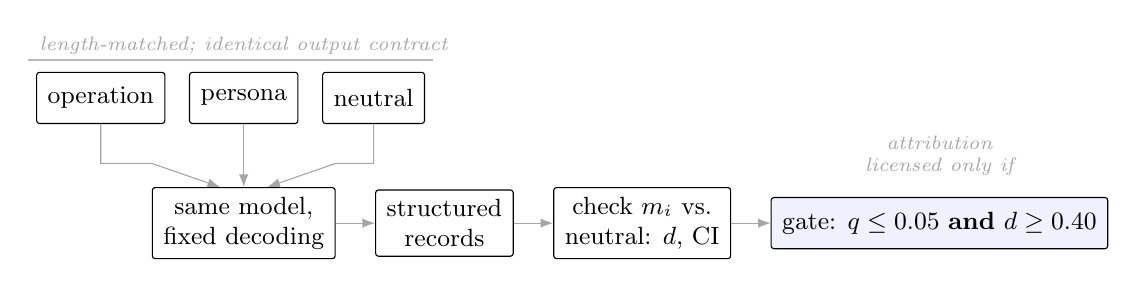
\begin{tikzpicture}[
  font=\small,
  box/.style={draw, rounded corners=1pt, minimum height=6.5mm, inner xsep=4pt, align=center},
  gate/.style={draw, rounded corners=1pt, fill=blue!6, minimum height=6.5mm, inner xsep=4pt,
               align=center},
  arr/.style={-{Latex[length=1.6mm]}, gray!70},
]
  \node[box] (op)      {operation};
  \node[box, right=3mm of op]  (pe) {persona};
  \node[box, right=3mm of pe]  (ne) {neutral};

  \node[gray!70, font=\scriptsize\itshape, above=1mm of pe.north]
        {length-matched; identical output contract};
  \draw[gray!55] ([xshift=-1mm,yshift=1.5mm]op.north west) -- ([xshift=1mm,yshift=1.5mm]ne.north east);

  \node[box, below=8mm of pe] (model) {same model,\\fixed decoding};
  \node[box, right=5mm of model] (rec) {structured\\records};
  \node[box, right=5mm of rec]   (chk) {check $m_i$ vs.\\neutral: $d$, CI};
  \node[gate, right=5mm of chk]  (gate) {gate: $q \le 0.05$ \textbf{and} $d \ge 0.40$};

  \node[gray!70, font=\scriptsize\itshape, align=center, above=1.5mm of gate.north]
        {attribution\\licensed only if};

  \draw[arr] (op.south) |- ([yshift=3mm]model.north west) -- ([xshift=-3mm]model.north);
  \draw[arr] (pe.south) -- (model.north);
  \draw[arr] (ne.south) |- ([yshift=3mm]model.north east) -- ([xshift=3mm]model.north);
  \draw[arr] (model) -- (rec);
  \draw[arr] (rec)   -- (chk);
  \draw[arr] (chk)   -- (gate);
\end{tikzpicture}
\caption{The check pipeline instantiated each role via three system prompts sharing one output
contract (the predeclared processing instruction, the role label alone, and no instruction at all).
All three traverse an identical path, so the contrast at the end isolates the prompt, and the gate
decides whether a benchmark delta may be read as an effect of the operation at all.}
\label{fig:pipeline}
\end{figure}

\subsection{Three prompt variants}
\label{sec:variants}

We present three conditions: operation vs neutral, which is the key contrast, and a persona
condition that disentangles the role condition from the operation it represents. We programmatically
test that all control conditions are padded so their length is within 10\% of the operation prompt
(to ensure that only the operation is helpful, not longer token strings), that our persona
conditions provably do not contain any words from the operation, and assert that none of the prompts
(when rendered) contain any medical terms. In all cases, we use a standardized structured output
format (a single JSON block with answer, abstain, confidence, list of atomic statements with whether
they have evidence, counterevidence and failures), which is necessary to enable all conditions to be
evaluated by the same set of metrics (the costs of this approach are discussed in
\S\ref{app:concedes}).

\subsection{The six checks}
\label{sec:six-checks}

For each condition, we specify a manipulation check. These manipulation checks (rate of
counterclaims and flags, number of contradictions found (corrected for abstention), number of atomic
statements made, diversity $\times$ concentration of hypotheses, number of sourced and unsourced
alternatives proposed and negative expected calibration error (NECE)) were all explicitly specified,
prior to data collection, by condition, and are only properties of the transformation represented by
the condition rather than the ``correctness'' of a solution (see Appendix~\ref{app:checks} for
details on how these checks are calculated).

\subsection{Decision rule and gate}
\label{sec:gate}

The checks are paired at the item level (the same item under all three variants) and per-item
differences are bootstrapped over 2,000 resamples. Both conditions in Figure~\ref{fig:pipeline} gate
on the number of observations, $n = 200$ --- a tight interval around a negligible difference will
pass a significance-only rule, and a large standardized effect with an interval spanning zero will
not offer evidence for a difference. The threshold is on a standardized but not absolute scale
because the six checks have no common unit (two return unbounded counts, one a rate difference in
$[-1, 1]$, one a distinct-item count). A single absolute threshold would be uninterpretable. Bounded
rates are sensitive to their inputs; rounding errors can seem like large moves.

The check runner exits non-zero if any of the roles fail to pass their checks, making them a gate on
a collection run instead of a report that will be produced and not read. If a role fails, it means
that this role hasn't validated the predeclared behavioural signature of its operation ---
equivalently, no matter how good it scored on the benchmark, this delta isn't licensed as evidence
for an effect of this operation.

\section{Experimental Setup}
\label{sec:setup}

\subsection{Pre-registration}
\label{sec:prereg}

We registered hypotheses, effect sizes, arm definitions, decision rules, and per-role predictions
before data collection. Two amendments were applied predating the data they're related to.
Specifically, amendment A2 claimed that improvement on the manipulation check was our primary
outcome, rather than the benchmark gain. A3 acknowledges a pilot which led to the analysis of the
47-item test split and pre-registered Benjamini--Hochberg control for the six role checks.

The registered decision rule is conjunctive. A role passes only if its paired
operation-versus-neutral contrast survives FDR control at $q = 0.05$ across the six-role family
\emph{and} reaches $d \ge 0.40$; a role is recorded as moving a benchmark only above a
leave-one-out contrast of 0.05. All intervals are 95\% paired bootstrap intervals over 2,000
item-level resamples. The scoped study is underpowered for the original council-gain hypothesis by
design --- at $n = 1{,}000$ the detectable effect is $\approx 0.048$ against a SESOI of 0.03 --- so
that hypothesis is reported as \textbf{not tested}, never as a null. The manipulation check is
differently placed: at $n = 200$ paired, the minimum detectable effect at 80\% power is
$\approx 0.20$, so the registered $d \ge 0.40$ threshold sits comfortably above the detection floor.

\subsection{Arms and cost matching}
\label{sec:arms}

The registered design has four arms: a full-operation council, a persona-label-only council, a
length-matched neutral council, and a cost-matched single-agent baseline. The council arms differ
only in the prompt (\S\ref{sec:variants}); model, decoding, output contract, and aggregation are
identical.

\textbf{The fourth arm was collected, but not as registered.} The registered baseline was
cost-matched. So, what we ran is the single-agent arm on the same model the councils use with one
direct call, making it neither cost-matched nor call-matched to the councils. The preregistered
cost-matched contrast remains uncollected. A council deficit against this baseline is therefore a
deficit against something that also costs less: a stronger practical claim and a weaker answer to
the registered question. \S\ref{sec:attribution} states the consequence for the attribution
baseline.

Two benchmarks are collected, both materialised by script from pinned immutable revisions and
verified by content hash so the corpus is reproducible byte-for-byte: HaluEval's QA split
\citep{li2023halueval} at \texttt{207f479c}, expanded to 20,000 binary items, and TruthfulQA's
generation split \citep{lin2022truthfulqa} at \texttt{741b8276}, 817 items. We use both for
non-commercial research evaluation, following the terms stated in their licenses. No personal data
is contained and we redistribute with the original license with attribution, with license
identifiers and URLs recorded per benchmark in \texttt{data/materialize\_manifest.json}.

\textbf{Accuracy analysis is limited to HaluEval.} Because the TruthfulQA generation split does not
provide an answer index (grading uses a judge model), the gold answer index is necessarily undefined
for all TruthfulQA questions. We classified TruthfulQA as free-form in preprocessing but did not
recognise before collection that the registered accuracy analysis needs a gold answer index, which
the generation split lacks. Examples from the TruthfulQA benchmark are, however, reflected in
behavioural metrics shown in \S\ref{sec:results} (e.g., refusal, abstention rates). All accuracy
metrics are, in turn, limited to HaluEval and reported as such (total examples), everywhere it
appears. For the benchmark arms, we use 1,000 HaluEval examples per arm (see
Appendix~\ref{app:splits}).

\subsection{Models}
\label{sec:models}

For our benchmark arms, we host \texttt{gpt-5.6-terra} in Microsoft Foundry (eastus2 Global
Standard), and for cross family replication in \S\ref{sec:replication} we host \texttt{grok-4.3} in
the same. Our pre-registered cost-matched arm uses \texttt{gpt-5.6-luna}, but as we switch Luna in
the collected single agent arm to Terra (\S\ref{sec:arms}), results do not include Luna. For all
arms and roles, we use \texttt{temperature=0}, 1,024 output tokens, \texttt{seed=1337},
\texttt{timeout=120s}. Of all provenance facts, only the following two are asserted (not inferred)
--- and only these two: (i) We specify the deployment name as the ID in our records. This deployment
is known to have used model version \texttt{2026-07-09}. The deployment name does not reference this
version: we thus specify the version in the manifest and do not attempt to infer it from the records
themselves; (ii) We specify the serving route (vendor, region, deployment mode), not infer it, since
our collection script accepts a provider argument. All other provenance facts are inferred (prompts
via hash, simulated/reality from provider attestation, splits by content).

\paragraph{Compute.}
All model calls were hosted as API calls, without using any GPU cluster nor hardware on the
provider's side. In collection, we issued 35,700 model calls. This includes three council arms at
1,500 items each $\times$ 6 different roles, another single agent arm at 1,500 items, and then three
prompt conditions at 200 items $\times$ 6 roles in each of \texttt{gpt-5.6-terra} and
\texttt{grok-4.3}. 35,208 (2.2\% absent rate) returned usable records, with recorded usage totalling
about 8.09M output tokens (\$128.66). Each arm in the council costs six calls per item: around 3,350
input and 1,428--1,659 output tokens per item (\$0.0239--\$0.0267), with mean per-agent latency at
3.1--4.5\,s; the single-agent baseline averages 2.44\,s (median 2.23\,s) and \$0.001792 per call.
Per-run cost, token, and latency breakdowns are in each run's \texttt{evaluation.json} under
\texttt{cost}. The synthesizer is the only trained component: 81--108 optimizer steps, 34.7--55.3\,s
wall clock per run on one Apple Silicon laptop (MPS, no CUDA). Every analysis in this paper re-runs
from the shipped records in under a minute on the same machine, with no API access.

\subsection{Attribution estimator}
\label{sec:attribution}

\textbf{In this work, we specify the value of the empty coalition.} As specified in our pre-reg, we
define $v(\emptyset)$ as the direct answer base model evaluated on identical per-sample inputs, with
records provided by the single-agent arms and joined into our council records. Note that we are able
to join 1,134/1,500 records per arm (including all 1,000 scorable records): we do not infer missing
values for 366 TruthfulQA records where the baseline abstained (or returned free-form text with no
answer index), we simply report these as missing. (Either way, leave-one-out does not consider the
empty coalition at all.)

For per-role attribution we perform leave-one-out by retraining on each coalition (seven trainings
total rather than the 64 required for a full Shapley computation, which is computationally
prohibitive at this scale; using a masking approximation to improve tractability deviates from
retraining by more than the effect size of interest, see Appendix~\ref{app:attribution-failures}).
Explicitly, leave-one-out is not a Shapley value and we do not claim it to be: in particular, it is
not efficient, so per-role contributions do not have to add up to $v(A) - v(\emptyset)$, and it
attributes all role--council interactions to each role. Writing $v$ in Harsanyi dividend form
$v(S) = \sum_{\emptyset \ne T \subseteq S} d(T)$, leave-one-out evaluates to
$v(A) - v(A \setminus \{i\}) = \sum_{T \ni i} d(T)$ while the Shapley value is
$\sum_{T \ni i} d(T)/|T|$, so the two differ by
$\sum_{T \ni i,\, |T| \ge 2} \frac{|T|-1}{|T|} d(T)$: the standalone term $d(\{i\})$ cancels and
leave-one-out charges role $i$ the whole of each interaction rather than its $1/|T|$ share.
Substitutable roles are negative dividends, so under the pairwise substitutability registered in
advance this difference is negative and every leave-one-out contrast is biased downward relative to
the Shapley value. The sign is imported rather than measured --- the seven coalitions evaluated here
do not identify $d(T)$ for $|T| \ge 2$ (Appendix~\ref{app:third-finding}) --- but the bias runs
against a positive verdict either way, so a role exceeding the 0.05 leave-one-out (LOO) threshold
has passed a conservative test.

Provenance is derived rather than asserted. Refusals, truncations, malformed responses, and retries
are counted and published per role rather than imputed. In the pilot and manipulation-check runs
reported here, those rates are zero across 1,128 pilot calls and the 3,600 calls; the benchmark arms
refuse only on TruthfulQA items, entering no accuracy contrast (Appendix~\ref{app:refusal}).
Appendix~\ref{app:provenance} gives the mechanism.

\section{Results}
\label{sec:results}

\subsection{Did the roles fire?}
\label{sec:did-fire}

In Figure~\ref{fig:checks} we perform the check for each role against the length-matched neutral
condition on 200 development items, in a paired bootstrap with 2,000 resamples (and no missing data,
across all 3,600 invocations). \textbf{Only one in six roles accomplishes its stated operation:}
counter-evidence checking more than doubles the rate of counterclaims and flagging relative to a
length-matched neutral instruction ($d = 1.03$). This check is a sum of two components and they do
not move together: explicit counterevidence items rise ($d = +1.48$ here, $+0.95$ on the second
family) while flagged claims fall, significantly so on the second family ($d = -0.33$).
Appendix~\ref{app:robustness} decomposes every check that has two parts.

\textbf{Two registered statistics are negative.} The explore-then-prune condition results in
\emph{less} hypothesis diversity compared to one with no explicit instructions ($d = -0.95$). The
local-claim checker finds \emph{fewer} claims compared to no explicit instructions ($d = -0.18$),
but its guard is effectively constant (1,191 of 1,200 records; invariant in every operation arm), so
we report but do not interpret this statistic as a validated reversal. As shown in Panel~(b), the
companion factor is saturated in both product rules. Thus explore-then-prune reflects a genuine
reversal rather than a within-metric tradeoff, while local-claim effectively collapses to a
one-factor check; Appendix~\ref{app:concedes} records this limitation.

\textbf{Three roles are statistically indistinguishable from neutral} ($|d| < 0.07$, $p > 0.36$).
\emph{Note: the null distribution for the rare hypothesis check does not reflect the full strength
of its safeguard against hallucinated hypotheses, which is based on the difference between unsourced
and sourced statements. Because sourcing approaches saturation in these records, this safeguard has
no effect, and the null is not as strong a baseline as for a check where the safeguard was
effective.}

\begin{figure}[t]
\centering
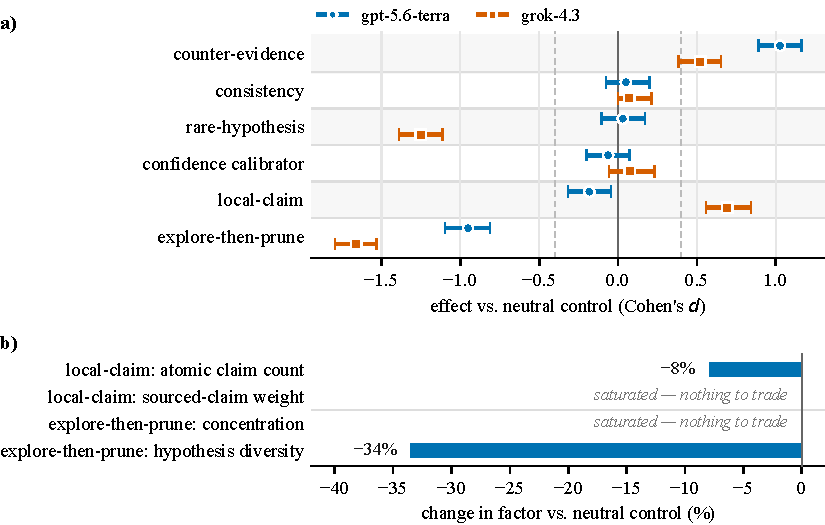
\includegraphics[width=\linewidth]{figures/checks_panel.pdf}
\caption{(a) Standardized difference of stated role effect against length-matched neutral condition,
on 200 datapoints, in two pretraining families, with 95\% bootstrap confidence intervals. Dashed
lines at pre-registered $|d| \ge 0.40$. (b) These flips are not tradeoffs because both measures are
product rules, with the factor being traded against pinned to maximum in both arms of the
experiment, leaving all the action to the factor we told it to increase.}
\label{fig:checks}
\end{figure}

\begin{table}[t]
\centering
\small
\begin{tabular}{llll}
\toprule
Check & Degeneracy named & Audit & Status \\
\midrule
counter-evidence      & ---                      & no guard was specified            & unguarded \\
consistency           & flag all, then abstain   & flag all and \emph{answer} scores 1.0 & defeatable \\
confidence calibrator & lower confidence blindly & constant shifts lower ECE         & defeatable \\
local-claim           & emit unchecked claims    & constant in 1,191/1,200 records   & collapsed \\
explore-then-prune    & breadth without resolution & concentration $\approx 1$ throughout & inactive \\
rare-hypothesis       & fabricate alternatives   & penalty $\approx 0$ throughout     & unexercised \\
\bottomrule
\end{tabular}
\caption{Each check's guard against the strategy it was written to exclude. Three failure classes
appear: guards that never vary, guards a cheap strategy defeats, and a check with none.}
\label{tab:guards}
\end{table}

\subsection{Auditing the guards}
\label{sec:audit}

A check is only as informative as the guard meant to stop a degenerate strategy passing it. We
stress-tested each against the strategy it names (Table~\ref{tab:guards});
Appendix~\ref{app:concedes} works the defeatable cases through.

\textbf{These audits were not pre-registered and do not replace the pre-registered check statistics;
they constrain their interpretation.} The statistics in \S\ref{sec:did-fire} stand; what the audit
withdraws is the licence to read them as construct-valid measurements --- including the one that
passes, which has no guard against fabricated counterevidence.

\subsection{The pattern replicates across families}
\label{sec:replication}

We designed these checks under a major assumption not yet verified: that the findings generalize
across models, and reflect something about the role prompting approach. To test this, we replicated
all six checks on the same 200 development examples for another pretraining family
(\texttt{grok-4.3}). The results are plotted in Figure~\ref{fig:checks}(a).

\textbf{The overall finding replicates.} The general finding that most role prompts do not score
well on their own check (one out of six, and two out of six) \emph{is} a property of the role
prompting approach at this scale, not just of a single model. Setting aside the local-claim check,
whose guard is constant in 1,191 of 1,200 records and which we therefore do not treat as a validated
instrument (Appendix~\ref{app:concedes}), the count is one of five on both families. The flip
replicates and becomes more pronounced: in both pretraining families, the \emph{explore-then-prune}
approach yields lower hypothesis diversity than a prompt specifying no particular approach, now with
a $d = -1.66$ on the second model as well. The single exception replicates as well: in both cases,
the only effective role was that of checking for counter-evidence.

\begin{table}[t]
\centering
\small
\begin{tabular}{lp{0.44\linewidth}l}
\toprule
 & does not move the benchmark & moves the benchmark \\
\midrule
passes its check & counter-evidence checking & --- \\
fails its check  & consistency checking, local-claim checking, explore-then-prune,
                   rare-hypothesis checking, confidence calibration & --- \\
\bottomrule
\end{tabular}
\caption{Registered two-axis classification across all six roles. The right-hand column is empty
because no role clears the pre-registered 0.05 leave-one-out threshold. Due to that, no role moved a
benchmark score \emph{without} passing its operational check --- a statement the check makes
available and a benchmark delta alone cannot. The local-claim row is retained for pre-registration
transparency; \S\ref{sec:audit} withdraws its instrument-level interpretation.}
\label{tab:twoaxis}
\end{table}

\textbf{Which roles fire does \emph{not} replicate.} Two of six change sign. Local claim checking
fails for one of these, and succeeds for the other. Rare hypothesis checking has no effect for one
of these and is highly reversed for the other. These are large effects. None of this difference is
due to one group being noisier than the other; three of these differences survive correction
($q = 0.016, 0.00075, 0.00075$). The one exception is the rare-hypothesis checking on
\texttt{gpt-5.6-terra} ($q = 0.71$), the null reported above. On the five checks we treat as
validated, this is one of five rather than two of six: local-claim checking is the other sign
change, and its reversal is a property of a check that reduces to a bare claim count, so the
non-transfer rests on rare-hypothesis checking alone. That remains a large non-transfer (null on one
family and $d = -1.25$ on the other) but it is one role, not two.

This is the strongest available argument for the tool. Had every role failed everywhere, the finding
would reduce to a list of prompts to avoid. Because at least one validated role-specific check
differs substantially across the two families tested, role behaviour should be validated on the
target model rather than assumed to transfer. We report two families and claim nothing about a
third.

The pre-registered binary classification --- does the role pass check, does it affect the benchmark
(Table~\ref{tab:twoaxis}) --- ends up in a single cell. The interpretation of this cell depends on
the asymmetry reported in A2.5. If a role affects the score \emph{despite} failing the check, this
is direct evidence for the claims of this paper --- an effect on the benchmark which is decoupled
from the claimed function. If a role \emph{passes} the check and has no effect, then this is a less
clear signal, as it is muddled with the detection issue (our detectable effect size at
$n = 1{,}000$ is 0.048, with SESOI 0.03; there could still be an effect which is just below the
floor).

Our pre-registration specifies that differences between arms should be reported as absolute effects,
rather than relative to some unknown gain (see Appendix~\ref{app:cross-arm}). These are informative
nulls, rather than inconclusive studies: with intervals of half-width $\approx 0.01$, we can be
confident that the full operational instructions prompt provides less than $\approx 1$ accuracy
point relative to either the operation names prompt or no operation, and the two operation prompts
have a zero difference. Similarly, the trained synthesiser also finds no extra value (see
Appendix~\ref{app:synth}).

\textbf{The only statistically detectable behavioural difference across arms is refusal, and it does
not affect these contrasts.} We never see refusal from an agent role on any HaluEval question in any
arm, so the comparisons are all across a constant, full set of questions. Refusal occurs only on
TruthfulQA, where the persona names prompt rejects significantly less than both controls: the mere
presence of a name can affect rejection rates with no distinct operation to attribute it to --- the
confounding mechanism we raise concern about in this paper, observed only on unscored questions
(Appendix~\ref{app:refusal}).

\textbf{There is no difference between council and single call.} Councils always perform \emph{worse}
than a single direct model query on all 1,000 scored questions, by $-0.015$ to $-0.022$ points, with
corrected intervals excluding zero. The effect sizes are smaller than H1's pre-registered 0.03
SESOI, so we claim councils do not outperform a single call, not that they are meaningfully worse;
and our baseline is a same-model single-call baseline rather than cost-matched (\S\ref{sec:arms}).
Appendix~\ref{app:single-call} gives both tie rules.

\textbf{Agents give high-confidence predictions whether they are correct or not.} Average reported
confidence is 0.982 against actual accuracy of 0.848, yet confidence is meaningfully associated with
correctness (AUROC 0.716) --- real signal squashed into the highest percentiles. Reported confidence
carries information about answer correctness but does not validate execution of the requested
operation (\S\ref{sec:did-fire}). The squashing is lineage-specific. \textbf{Exploratory}, not
pre-registered (Appendix~\ref{app:confidence}).

We perform the pre-registered attribution study via leave-one-out retraining of all candidates (full
council vs.\ six different drop-one coalitions, seven trainings total, see
Appendix~\ref{app:loo} for details). \textbf{No role makes a difference.} The maximum leave-one-out
difference in magnitude is 0.016, well below the pre-registered threshold of 0.05 (less than a third
as large), and all ranges include zero. These results are essentially null (5 different values for
different coalitions, so not a degeneracy) but also directionally biased toward zero (leave-one-out
penalizes every interaction with the council with that role, skewing differences down, making them
conservative) and none are near the threshold such that the conservative bias would be relevant.

\textbf{For one of the two pre-registered tests, we have no data.} The FDR family testing agent-role
pairs against their primary benchmark assigns one role (the one role whose primary benchmark
survived scoping) to TruthfulQA --- upon which it scores zero. Half of this FDR family's cells are
missing, meaning the corrected $q$-values are indeterminate and we do not report them (rather than
just returning the HaluEval column).

We do not (and do not report null findings for) the primary council-improvement hypothesis or H2.
The scoped analysis is, by design, underpowered to detect the primary hypothesis. Similarly, for
five of six roles, their pre-registered primary target is removed by the dual-benchmark reduction;
the LOO results are thus per-role results on HaluEval, which is no role's pre-registered primary
target. Finding one for H2 would be precisely the kind of result-switching we oppose in this work.
For the manipulation checks only, the results generalise across families. Only one family has data
for the two benchmarks, LOO analysis, or single-call comparison.

\section{Limitations and Claims This Paper Does Not Make}
\label{sec:limitations}

\paragraph{Limitations in scope.}
We validate our manipulation checks on another pretraining family (\S\ref{sec:replication}).
However, our benchmark comparisons, leave-one-out analysis, and single call comparison are only
performed within a single pretraining family with a similar level of capability. Validation on a
second family only establishes replication, not population-level generalization. We also only
examine two benchmarks, both in English.

\paragraph{Limitations in measurement.}
All our arms return the same format; this means our manipulation checks are measuring the relative
difference rather than the existence of these factors, resulting in lower contrast relative to an
experiment where the null condition doesn't return anything. The concentration and sourced claim
manipulation checks were designed as two-factorial but effectively function as a one-factorial
design since both conditions are saturated; this collapses their corresponding statistics. We only
filter refusals in TruthfulQA, where there is no individual question contributing to the accuracy
comparisons (Appendix~\ref{app:refusal}). While the role priming could influence whether the model
refuses to answer at all, it did not affect that measured benchmark in our experiment.

\paragraph{Limitations in provenance.}
We directly state, but cannot verify, two pieces of information (\S\ref{sec:models}). First, we
state the model variant but it cannot be deduced from the serving name. Second, we state the serving
path but it cannot be deduced from the manifest since our scraper does not record provider. We
conducted an experiment on a 47-question test dataset before our registered analysis; no out-dated
correction affected a registered quantity, and we ask the reader to consider any analysis they
believe affected to be exploratory. Our analysis of failure modes in attribution are only evaluated
on simulated data in Appendix~\ref{app:attribution-failures} to serve as evidence of existence and
possible mechanisms rather than rates of failure in public models.

\paragraph{What this does not claim: beating baselines.}
This scoped experiment isn't powered for that. We also don't claim to have found correspondences
between LLM capabilities and clinical constructs; this was only inspired by that analogy. We do not
claim to be the first to do this work; we just note that role checks are rarely done. We don't track
how often attribution errors occur. We did not test H1 (not powered by design) nor H2 (lost its
target when we applied the two benchmark simplification and did not choose an alternative contrast
such as HaluEval); provide cost-matched comparisons of council vs single agent: we recorded a
same-model single-call arm, 6$\times$ cheaper; to calibrate: we do not propose a calibration
procedure, Appendix~\ref{app:confidence} is a gap analysis rather than a solution. Finally, we do
not claim that capability is broken when the constraint that we provided is lifted; this requires
training tests we didn't run.

\paragraph{Solely for research.}
Nothing here licenses deployment. The council described in this paper must not be used for medical,
legal, financial or other consequential decisions on the basis of benchmark accuracy.


\bibliographystyle{plainnat}
\bibliography{references}

\newpage
\appendix
\section{Synthesiser estimator}
\label{app:synth}

The cross-arm analysis using only majority vote is given in Appendix~\ref{app:cross-arm}. That
analysis is cleaner --- no training is used and any difference between arms is due to the prompt
difference only (the synthesiser used a separate trained model for each arm, inflating its variance
with training variance in addition to the prompt). The majority-only analysis is relegated to the
Appendix because it does not alter any of our conclusions.

For the synthesiser accuracies on 184 test problems, we get 0.783 (op), 0.804 (pl), and 0.799
(neutral). None of the contrasts between any two arms excludes zero: the op--pl contrast is $-0.022$
($[-0.065, +0.022]$, $q = 0.85$), the op--neutral contrast is $-0.022$ ($[-0.065, +0.027]$,
$q = 0.85$), and the pl--neutral contrast is $+0.005$ ($[-0.027, +0.038]$, $q = 0.88$). The
point-estimates rank the operation arm lower than the controls, with the opposite ranking as with
majority voting, but the $\pm 0.05$ size of the confidence intervals at $n = 184$ exclude any
ranking.

The operation arm's synthesiser accuracy is not significantly different from the baselines it is
designed to outperform: there is no difference to pure majority voting ($\Delta = 0.000$) and the
biggest difference between the synthesiser and any one of the six single agents is 0.027 in absolute
value, with the confidence interval including zero. From \texttt{runs/cross\_arm.json} and
\texttt{runs/arms-cca\_council/evaluation.json}.

\section{Provenance and exclusion accounting}
\label{app:provenance}

We leave provenance to be inferred: providers self-report whether their answers are fabricated
(omitted answers are treated as synthetic to guarantee that a buggy provider logs simulated, not
real, records; if any provider is synthetic, the record is synthetic; and the analysis step simply
skips simulated records); track and report refusals, truncation, malformed outputs, and retried
queries by role (rather than assuming them); and omit rows without a record in any variant from
contrasts by role (rather than assuming them to be zero).

We report no refusals, no truncations, no malformed outputs, and no retried queries in our current
experiments: we encountered none in 1,128 pilot queries or 3,600 queries in the manipulation check
study.

\section{Scope of the novelty search}
\label{app:novelty-search}

We only used nine queries to arXiv, ACL Anthology, OpenReview (rejected and withdrawn papers), and
Semantic Scholar and only performed title/abstract screening, did not obtain full-texts nor snowball
through citations, nor queried PubMed by clinical MeSH terms, nor even had a double screener to
report inter-screener agreement on, reported only five out of eight queries to Semantic Scholar that
encountered rate limits as failures (rather than as zero findings), already encountered two
potential predecessors and one borderline finding (\S\ref{sec:related}) and thus claim no ``none in
$N$ papers screened''.

\section{What the check design concedes}
\label{app:concedes}

Three concessions were predeclared; a fourth was identified by post-collection audit and is reported
here.

\paragraph{The shared output contract compresses the contrast.}
To all versions we explicitly request atomic claims, counterclaims, and fault indicators in their
output. This means that even the length-matched neutral condition will output some counterclaims. In
that case we can only check for quantity, not for existence. While the dynamic range persists, it
will be squeezed compared to a setting where the neutral version did not output such information. We
anticipate operation $-$ neutral gaps to be smaller than with a version of this experiment that did
not employ a common record format but viewed the standard record format as necessary to route all
treatments through the same measurement apparatus.

\paragraph{Absent records are excluded, never scored as zero.}
We do not impute missing values, i.e.\ in case of refusals, truncations, or other malformations.
Otherwise we would artificially deflate the check scores in line with the failure rate, rather than
the performance of the variations.

\paragraph{The checks are benchmark-independent.}
A check only evaluates if the model lived up to its role, but does not evaluate the utility of the
role. For this reason shrinking the scope from four to two benchmarks is cost-neutral: it comes at
the expense of losing a role-wise distinction on a designated primary benchmark, not any roles.

\paragraph{The local-claim guard collapsed, and the check is therefore one-factorial in fact.}
\texttt{\_check\_claim\_decomposition} scores atomic claims per record weighted by the fraction
carrying a local check, so the weighting term is the guard: a role that emitted many unchecked
claims should not score well. In the collected records that term is the constant 2.0 in 1,191 of
1,200 records and has no variance at all in the operation arm of either family
(Table~\ref{tab:localclaim-guard}). The check is thus $2\times$ the claim count, and its guard never
discriminated. We report all local-claim results for preregistration transparency, but do not
interpret them as a validated pass or reversal.

\begin{table}[h]
\centering
\small
\begin{tabular}{llrrrl}
\toprule
Family & Arm & $n$ & weight $= 2.0$ & weight $< 2.0$ & distinct values \\
\midrule
\texttt{gpt-5.6-terra} & operation & 200 & 200 & 0 & \{2.0\} \\
\texttt{gpt-5.6-terra} & persona   & 200 & 200 & 0 & \{2.0\} \\
\texttt{gpt-5.6-terra} & neutral   & 200 & 200 & 0 & \{2.0\} \\
\texttt{grok-4.3}      & operation & 200 & 200 & 0 & \{2.0\} \\
\texttt{grok-4.3}      & persona   & 200 & 197 & 3 & \{1.667, 2.0\} \\
\texttt{grok-4.3}      & neutral   & 200 & 194 & 6 & \{1.667, 2.0\} \\
\bottomrule
\end{tabular}
\caption{The local-claim check's source-weighting guard, by family and arm. The guard takes one value
in 1,191 of 1,200 records and is constant in every operation arm, so the product it belongs to has
only one live factor.}
\label{tab:localclaim-guard}
\end{table}

\paragraph{Two further guards are defeatable rather than collapsed.}
The consistency safeguard evaluates flag rate against abstain rate. This means that the behavior of
always-flagging but never-abstaining gets a perfect score of 1.0 (compared to the operation prompt
score of 0.025). This safeguards against always-flagging-and-abstaining, but not
always-flagging-and-responding. The calibration safeguard was designed with the assumption that
uniformly reducing confidence would not reduce the expected calibration error. However, in this
dataset, we see that uniformly reducing confidence by a constant for all samples reduces ECE from
0.144 to 0.112 ($-0.05$ on the operation arm), and from 0.129 to 0.065 ($-0.10$ on the neutral arm),
without actually performing any calibration based on individual samples. While neither of these were
pre-registered, they do put limitations on how you can interpret their corresponding safeguard
metric in \S\ref{sec:did-fire}, but they do not supplant the safeguard metric.

\section{Benchmark materialisation and splits}
\label{app:splits}

We split the data 50/15/15/20 train/calibration/validation/test by calculating the salted hash of the
item contents. We further sample 200 items from the train split to be used for a manipulation-check
dev set.

We draw 1,000 HaluEval samples per arm for the benchmark arms, sampled sequentially from the file.
Sampling sequentially is not correlated with the data split (which is calculated off of item
content, not file index), and we have confirmed that the proportions of items in each split of the
subsample are within 1 percentage point of those in the full corpus.

\section{Failure modes in coalition attribution}
\label{app:attribution-failures}

If manipulation checks are an assessment of whether each role followed its instructions, this section
evaluates whether the attribution system followed its instructions: did the attribution system
calculate that a role's contribution to a coalition ablation was $\phi$, or does it vouch for
hallucination? We present two ways that this fails, discovered by running code that we had written
but not executed. Two are from our system presented as existence proofs with explanations of
mechanism, not prevalence in the wild.

\subsection{Finding (i): an all-zero ablation that passed its own efficiency check}

When we ran a Shapley ablation in retrain-per-coalition mode, it completed all 64 coalitions without
error and returned identically zero contributions for every role, while the efficiency axiom --- the
standard internal correctness check for a Shapley computation --- reported no violation.

\begin{table}[h]
\centering
\small
\begin{tabular}{lrr}
\toprule
 & retrain & masked (same config) \\
\midrule
Distinct coalition values across 64 & 1 & 30 \\
$v(\emptyset)$ & 0.0000 & 0.0000 \\
$v(A)$ & 0.0000 & 0.3314 \\
Every role's $\phi$ & 0.0000, CI $[0, 0]$ & $+0.036 \ldots +0.084$ \\
Efficiency check & 0.00e-00 (vacuous) & 0.00e-00 \\
\bottomrule
\end{tabular}
\caption{The degenerate ablation beside a masked run on identical configuration. The efficiency check
passes in both columns, and distinguishes them not at all.}
\label{tab:degenerate}
\end{table}

Why? We also found that we were reusing the same calibration data for all models. We had calibrated
the logit temperature and selective prediction threshold on the calibration set for the original
model trained on the main coalition dropout, and then reused this for all 64 models that are
independently retrained for each new data dropout. This meant the threshold was set way higher than
all selection scores, which are a completely new scale for each model, causing all to abstain and all
coalition values to be equal to the abstention credit (i.e., zero).

No overfitting was observed since efficiency (i.e., $\sum_i \phi_i = v(A) - v(\emptyset)$) will
always hold for $0 = 0 - 0$. Anything true for a non-degenerate answer is also true for a degenerate
answer; \textbf{this is the key learning, as internal checks can never catch a degenerate solution
because degenerate solutions are always internally consistent.}

The solution to this was to train each model in the ablation loop with its own logit temperature and
selective prediction threshold, both calibrated solely on the calibration set. Generalised learning:
when ablation involves retraining of a model, recalibrate all models. This is not a detail you can
cut corners on without completely breaking your analysis.

This guard is a different efficiency check --- a degeneracy check tallying distinct values assigned
to coalitions and loudly failing if the value function is degenerate. And indeed our scoped
experiment on real records now checks out, reporting 5 distinct coalition values:
\texttt{OK got 5 distinct coalition values}, a sanity check that the patched branch works correctly
on real data.

\subsection{Finding (ii): the masking approximation exceeds the effect it is used to detect}

With the calibration fixed, both estimator modes were run on identical configuration, differing only
in \texttt{shapley\_mode}. This isolates the masking approximation.

\begin{table}[h]
\centering
\small
\begin{tabular}{lrrr}
\toprule
Role & masked & retrain & gap \\
\midrule
\texttt{counter\_evidence\_checker} & $+0.0618$ & $+0.0356$ & $-0.0262$ \\
\texttt{consistency\_checker}       & $+0.0381$ & $+0.0510$ & $+0.0129$ \\
\texttt{local\_claim\_checker}      & $+0.0566$ & $+0.0711$ & $+0.0145$ \\
\texttt{explore\_then\_prune}       & $+0.0836$ & $+0.0607$ & $-0.0230$ \\
\texttt{rare\_hypothesis\_checker}  & $+0.0556$ & $+0.0560$ & $+0.0004$ \\
\texttt{confidence\_calibrator}     & $+0.0356$ & $+0.0570$ & $+0.0214$ \\
\midrule
\multicolumn{4}{l}{mean $|$gap$|$ 0.0164 \quad max $|$gap$|$ 0.0262 \quad SESOI 0.010} \\
\bottomrule
\end{tabular}
\caption{Per-role contributions under the two estimator modes. The mean disagreement between
estimators is larger than the smallest effect the pre-registration declares worth detecting.}
\label{tab:estimator-gap}
\end{table}

Two consequences follow, and both are properties of the estimator rather than of the data.

\textbf{The approximation error exceeds the target effect.} For per-role effect sizes smaller than
0.010 (the lowest effect size of interest in the pre-registration), the mean gap between the two
modes is 0.0164, so a masked experiment will not be able to report a per-role conclusion at the
effect size of interest in the pre-registration, regardless of the confidence interval.

\textbf{The ranks are not stable.} The \texttt{explore\_then\_prune} role ranks 1st and the
\texttt{counter\_evidence\_checker} role ranks 2nd according to the masked ranks, but after retrain,
the \texttt{local\_claim\_checker} ranks 1st and the \texttt{counter\_evidence\_checker} ranks last.
Statements like ``role X contributes the most'' are an artifact of the estimator and must be
calculated using retrain.

Interestingly, both modes give identical results on total values ($v(\emptyset) = 0.0000$ and
$v(A) = 0.3314$ both). So masking is fine for iteration and the total council comparison, but fails
where you use it most: the per-role breakdown. For this reason, in our scoping study we
pre-registered a leave-one-out retrain sweep as opposed to a mask mode sweep --- this wasn't designed
into the study; it resulted from the study.

\subsection{What they have in common}

Each of these was validated by the respective correctness checks of the whole pipeline. The
ablation's degeneracy passed the efficiency tests. The masked estimator validity test validated that
it constructed good confidence intervals around values that didn't survive the estimator swap. The
interaction table fit together perfectly and was in part an artifact of a modelling constant.

The theme is the same: \textbf{validity tests are validity tests, they can only check that something
is valid --- not whether it actually measured anything.} Each of these can only be done through an
orthogonal validity test; a validity test on variation, rather than coherence.

This is just \S\ref{app:concedes} meta. Just like you want a manipulation check before interpreting
the results of an intervention (did the intervention even happen?), you want a degeneracy check
before interpreting the results of a value function (did the value function vary?). In both cases the
problem will be silent, with the result being well-defined, and no internal validity tests along the
way will catch it.

\section{A third attribution finding, reported with its confound}
\label{app:third-finding}

Across all 15 role pairs, the pairwise interaction terms are negative and of the same order of
magnitude as the main effects, implying that the roles substitute for one another rather than
composing. We report this in full and decline to build on it, for a stated reason: our simulator
deliberately induces correlated common-mode failure, so the magnitude is partly downstream of a
constant we chose. We report the induced correlation parameter alongside the interaction table, and
we do not carry the finding into the abstract. It stays unpromoted, and the scoped study cannot
change that. The registered estimator there is leave-one-out, which contrasts the full council
against each drop-one coalition and never evaluates a pair in isolation; it therefore yields no
pairwise interaction term at all. Finding (iii) is consequently not testable on our real records
rather than tested and unconfirmed, and it remains a simulated-data observation reported for
completeness.

One real-record measurement is adjacent but is deliberately not offered as confirmation. In the
scoped run the mean pairwise error correlation across the six agents is 0.80 (max 0.95, on the 184
items every agent answered), which bounds how much independent evidence a six-agent council supplies.
That is a property of the agents' mistakes, not the estimator's interaction terms, and conflating the
two would be exactly the kind of substitution this paper argues against.

\section{Differential refusal}
\label{app:refusal}

None of these comparisons are affected by differences in refusal behaviour, which is the only
difference between the arms. There were zero refusals in any of the 6,000 agent slots in the HaluEval
benchmark in any of the arms, meaning that the HaluEval comparisons made above are comparing an
identical and complete set of answers (the table above is a perfect matching). The only refusals are
in the TruthfulQA questions, which are not scored (there is no gold answer for them), and also not
part of the accuracy comparisons: 6.1\% refusal rate for agent slots in the operation arm, 5.5\%
refusal rate for agent slots in the neutral arm, 4.5\% refusal rate for agent slots in the
persona-label arm. These differences in refusal rate between operation and neutral are not
significant ($+0.63$ pts difference, 95\% CI $[-0.57, +1.80]$, $q = 0.31$), but the persona-label
prompt has a significantly lower refusal rate than both of these ($-1.63$ vs operation $q = 0.006$,
$-1.00$ vs neutral $q = 0.035$). This shows that you can affect a model's willingness to answer a
question by appending just a role label to the prompt, an operation-less effect which is the other
pathway of concern in this paper, but we only see this in the unscored TruthfulQA questions, so we
don't include this effect in our results.

\section{Operationalisation of the six checks}
\label{app:checks}

Each check reduces a role's records to one scalar in which higher means more of the operation's
signature behaviour. The design problem is not measuring the behaviour but preventing a degenerate
strategy from scoring well on it, so each check carries a guard (Table~\ref{tab:check-specs}).

\begin{table}[h]
\centering
\small
\begin{tabular}{p{0.20\linewidth}p{0.38\linewidth}p{0.32\linewidth}}
\toprule
Role & Quantity measured & Guard \\
\midrule
counter-evidence checker & Counterevidence items plus claims flagged unsupported or contradicted,
per record & --- \\
consistency checker & Rate of contradiction and calculation-error flags, minus the abstention rate &
Cannot be passed by flagging everything and refusing to answer \\
local-claim checker & Atomic claims per record, weighted by the fraction carrying a local check &
Rewards decomposition that is checked, not decomposition alone \\
explore-then-prune & Distinct claim texts, multiplied by evidential concentration & Breadth alone
does not score; unresolved claims suppress it \\
rare-hypothesis checker & Sourced supported claims minus unsourced supported claims & Fabricated
alternatives subtract \\
confidence calibrator & Negative expected calibration error over declared confidences & Intended to
exclude blanket low confidence; see \S\ref{sec:audit} \\
\bottomrule
\end{tabular}
\caption{The six executable checks. Each is a predeclared function of the structured records; five
carry an explicit guard against a strategy that would otherwise satisfy the check without performing
the operation. \S\ref{sec:audit} reports which of those guards actually constrain that strategy.}
\label{tab:check-specs}
\end{table}

The essence of these designs is these guards. Since a consistency checker could always fire on all
questions and abstain from answering to achieve a high naive consistency detection rate, we subtract
its abstention rate from the consistency detection rate. Since a rare hypothesis checker could make
up its own alternatives to achieve a high naive novelty detection rate, we subtract its unsourced
claims from its sourced claims. Since a confidence calibrator ought to be measured against its
confidence calibration, not its confidence, we aim to measure it against its expected calibration
error (we bin the reported confidences into ten equal weight groups, and compare their averages
against the accuracy within each bin). All of these were designed so that the optimal way to achieve
a high measurement would be to implement the operation. We check how well they did that in
\S\ref{sec:audit}, though here they didn't do that well.

We pad both of these controls to the same length as the operation prompt when they are rendered such
that the 10\% margin of \S\ref{sec:variants} applies to each role independently, which we audit in
Table~\ref{tab:padding} where we see the maximum padding deviation across the twelve controls is
3.17\%. Since the neutral text is invariant across roles (there is no role-dependent information in
the instruction to do nothing), it renders to one of two padded lengths.

\begin{table}[h]
\centering
\small
\begin{tabular}{lrrrrr}
\toprule
Role & operation & neutral & persona & neutral dev. & persona dev. \\
\midrule
counter-evidence      & 1947 & 1997 & 1901 & 2.6\% & 2.4\% \\
consistency           & 1923 & 1862 & 1902 & 3.2\% & 1.1\% \\
local-claim           & 1896 & 1862 & 1906 & 1.8\% & 0.5\% \\
explore-then-prune    & 1938 & 1997 & 1905 & 3.0\% & 1.7\% \\
rare-hypothesis       & 1953 & 1997 & 1902 & 2.3\% & 2.6\% \\
confidence calibrator & 1952 & 1997 & 1909 & 2.3\% & 2.2\% \\
\bottomrule
\end{tabular}
\caption{Rendered system-prompt lengths in characters, per role. Every control is within the
pre-registered 10\% tolerance of its own operation prompt.}
\label{tab:padding}
\end{table}

Because the six statistics carry six different units, the standardized difference is what the
decision rule reads. Table~\ref{tab:raw-diffs} reports each check's raw operation-versus-neutral
difference beside it, in the units of that check, for both pretraining families.

\begin{table}[h]
\centering
\small
\begin{tabular}{llrrrr}
\toprule
 & & \multicolumn{2}{c}{\texttt{gpt-5.6-terra}} & \multicolumn{2}{c}{\texttt{grok-4.3}} \\
\cmidrule(lr){3-4}\cmidrule(lr){5-6}
Role & Check statistic & raw & $d$ & raw & $d$ \\
\midrule
counter-evidence      & counterclaim-and-flag rate           & $+0.6750$ & $+1.028$ & $+0.3950$ & $+0.522$ \\
consistency           & contradiction score net of abstention & $+0.0100$ & $+0.050$ & $+0.0050$ & $+0.071$ \\
rare-hypothesis       & sourced $-$ unsourced alternatives    & $+0.0250$ & $+0.031$ & $-1.0400$ & $-1.250$ \\
confidence calibrator & negative expected calibration error   & $-0.0141$ & $-0.063$ & $+0.0060$ & $+0.074$ \\
local-claim           & atomic claims (weighted)              & $-0.4000$ & $-0.182$ & $+1.8900$ & $+0.694$ \\
explore-then-prune    & diversity $\times$ concentration      & $-0.8550$ & $-0.951$ & $-1.3500$ & $-1.661$ \\
\bottomrule
\end{tabular}
\caption{Each check's raw operation-versus-neutral difference on the 200 development items, in the
units of that check, beside the standardized difference the decision rule reads. Rows are ordered as
in Figure~\ref{fig:checks}(a). Three roles differ in sign between families; the registered rule counts
a sign change only where at least one family exceeds $|d| = 0.20$, which is the two reported in
\S\ref{sec:replication}. Source: \texttt{runs/cross\_family.json}.}
\label{tab:raw-diffs}
\end{table}

\section{Robustness of the check verdicts}
\label{app:robustness}

Everything in this section is exploratory. The registered verdict is the conjunctive rule of
\S\ref{sec:variants} --- interval excluding zero and $d \ge 0.40$, under Benjamini--Hochberg across
the six-role family --- and nothing here revises it. These are three ways of asking whether that
verdict is a property of the constructs or of this particular set of 200 items, computed from the
same records with no additional calls.

\subsection{Sensitivity to the standardized threshold}

The registered threshold is $d \ge 0.40$. Table~\ref{tab:threshold-sweep} sweeps it. On
\texttt{gpt-5.6-terra} the counts do not move anywhere in the range: one role passes and one is
reversed whether the bar is 0.20 or 0.80, so ``one of six'' is not an artifact of the particular
value registered. On \texttt{grok-4.3} the counts are not stable: counter-evidence checking drops out
above 0.50, so the two-of-six figure there does depend on where the bar sits.

\begin{table}[h]
\centering
\small
\begin{tabular}{lrrrrrr}
\toprule
 & \multicolumn{3}{c}{\texttt{gpt-5.6-terra}} & \multicolumn{3}{c}{\texttt{grok-4.3}} \\
\cmidrule(lr){2-4}\cmidrule(lr){5-7}
$d$ threshold & pass & reversed & null & pass & reversed & null \\
\midrule
0.20          & 1 & 1 & 4 & 2 & 2 & 2 \\
0.25          & 1 & 1 & 4 & 2 & 2 & 2 \\
0.30          & 1 & 1 & 4 & 2 & 2 & 2 \\
0.35          & 1 & 1 & 4 & 2 & 2 & 2 \\
$0.40^\star$  & 1 & 1 & 4 & 2 & 2 & 2 \\
0.45          & 1 & 1 & 4 & 2 & 2 & 2 \\
0.50          & 1 & 1 & 4 & 2 & 2 & 2 \\
0.60          & 1 & 1 & 4 & 1 & 2 & 3 \\
0.70          & 1 & 1 & 4 & 0 & 2 & 4 \\
0.80          & 1 & 1 & 4 & 0 & 2 & 4 \\
\bottomrule
\end{tabular}
\caption{Role counts as the standardized threshold is swept. $\star$ marks the registered value.
Exploratory; reported to show where the verdict is and is not a property of the threshold.}
\label{tab:threshold-sweep}
\end{table}

\subsection{Stability of the qualitative verdict}

Table~\ref{tab:verdict-stability} recomputes each role's verdict over 2,000 item resamples and over
subsamples of half the items. Every role on \texttt{gpt-5.6-terra} keeps its classification in every
resample, and sits between 3.0 and 6.8 resample standard deviations from the $\pm 0.40$ boundary. The
one unstable cell is counter-evidence checking on \texttt{grok-4.3}: its resampled $d$ has a 95\%
interval of $[+0.374, +0.698]$, which straddles the threshold, and 7\% of resamples classify it as
indistinguishable. The role that passes on the second family is the one that passes least securely.

\begin{table}[h]
\centering
\small
\begin{tabular}{lllllll}
\toprule
 & \multicolumn{3}{c}{\texttt{gpt-5.6-terra}} & \multicolumn{3}{c}{\texttt{grok-4.3}} \\
\cmidrule(lr){2-4}\cmidrule(lr){5-7}
Role & verdict & agree & $n{=}100$ & verdict & agree & $n{=}100$ \\
\midrule
counter-evidence      & passes            & 100\% & 100\% & passes            & 93\%  & 93\% \\
consistency           & indistinguishable & 100\% & 100\% & indistinguishable & 100\% & 100\% \\
rare-hypothesis       & indistinguishable & 100\% & 100\% & reversed          & 100\% & 100\% \\
confidence calibrator & indistinguishable & 100\% & 100\% & indistinguishable & 100\% & 100\% \\
local-claim           & indistinguishable & 100\% & 100\% & passes            & 100\% & 100\% \\
explore-then-prune    & reversed          & 100\% & 100\% & reversed          & 100\% & 100\% \\
\bottomrule
\end{tabular}
\caption{Qualitative verdict over 2,000 paired item resamples, and over subsamples of 100 of the 200
items. ``Agree'' is the share of resamples returning the point verdict. Exploratory.}
\label{tab:verdict-stability}
\end{table}

\subsection{Component decomposition of every composite check}

Figure~\ref{fig:checks}(b) decomposes the two checks that are products. Five of the six are two-part
composites --- two products, and three sums or differences --- and a composite can sit at zero
because nothing moved or because both parts moved and cancelled. Table~\ref{tab:components}
separates them.

Two readings matter. The consistency and rare-hypothesis nulls on \texttt{gpt-5.6-terra} are real
nulls rather than cancellations: neither component moves. And the counter-evidence check, the one
role that passes, is a sum whose parts move in opposite directions --- explicit counterevidence items
rise while flagged claims fall, significantly so on \texttt{grok-4.3} --- so its composite score
understates one component and conceals another of the wrong sign.

\begin{table}[h]
\centering
\small
\begin{tabular}{lrrrrrr}
\toprule
 & \multicolumn{3}{c}{\texttt{gpt-5.6-terra}} & \multicolumn{3}{c}{\texttt{grok-4.3}} \\
\cmidrule(lr){2-4}\cmidrule(lr){5-7}
Component & neutral & operation & $d$ & neutral & operation & $d$ \\
\midrule
\multicolumn{7}{l}{\emph{counter-evidence (sum)}} \\
\quad counterevidence items & 0.305 & 1.020 & $+1.475$ & 0.470 & 1.015 & $+0.949$ \\
\quad flagged claims        & 0.305 & 0.265 & $-0.104$ & 0.205 & 0.055 & $-0.328$ \\
\multicolumn{7}{l}{\emph{consistency (difference)}} \\
\quad flag rate             & 0.015 & 0.025 & $+0.050$ & 0.000 & 0.005 & $+0.071$ \\
\quad abstention rate       & 0.000 & 0.000 & $+0.000$ & 0.000 & 0.000 & $+0.000$ \\
\multicolumn{7}{l}{\emph{rare-hypothesis (difference)}} \\
\quad sourced supported     & 2.290 & 2.315 & $+0.031$ & 2.550 & 1.495 & $-1.293$ \\
\quad unsourced supported   & 0.000 & 0.000 & $+0.000$ & 0.015 & 0.000 & $-0.123$ \\
\multicolumn{7}{l}{\emph{local-claim (product)}} \\
\quad atomic claim count    & 2.520 & 2.320 & $-0.182$ & 2.800 & 3.730 & $+0.685$ \\
\quad sourced weight        & 2.000 & 2.000 & $+0.000$ & 1.990 & 2.000 & $+0.175$ \\
\multicolumn{7}{l}{\emph{explore-then-prune (product)}} \\
\quad diversity             & 2.550 & 1.695 & $-0.951$ & 2.885 & 1.525 & $-1.669$ \\
\quad concentration         & 1.000 & 1.000 & $+0.000$ & 0.997 & 1.000 & $+0.100$ \\
\bottomrule
\end{tabular}
\caption{Each composite check split into its two components, per family. Means are per record.
Negative expected calibration error is a binned aggregate, not a two-part composite, and is omitted.
The rare-hypothesis guard (unsourced supported) is identically zero under both prompts on
\texttt{gpt-5.6-terra}, which is the saturation \S\ref{sec:did-fire} reports. Exploratory.}
\label{tab:components}
\end{table}

\section{Verbalised confidence against correctness}
\label{app:confidence}

Every agent returns a confidence with its answer. Across all 18,000 agent answers, mean stated
confidence is 0.982 against a realised accuracy of 0.848 --- a gap of $+0.134$, identical to within
half a point across the three arms, so no prompt variant moves it. This analysis is exploratory and
was not pre-registered.

The gap is not an absence of self-knowledge. Confidence discriminates correctness at AUROC 0.716, and
it does so monotonically: answers stated at 0.99, 79\% of the total, are 91.5\% correct; those at
0.98 are 67.2\% correct; those at 0.90 are 42.6\% correct. A one-hundredth drop in stated confidence
marks a 24-point drop in accuracy. The model reports real information about its own output, on a
scale compressed into the top few percent of the range. Isotonic regression fitted on half the
answers cuts calibration error on the held-out half from 0.133 to 0.007 while leaving AUROC on that
half untouched (0.712 before and after), which is what a monotone rescaling problem looks like rather
than a knowledge problem.

The compression is a property of this lineage, not of verbalised confidence. On the second family
(\S\ref{sec:replication}), over the same 3,600 check calls, stated confidence averages 0.869 with a
standard deviation of 0.067 and only 15\% of answers at or above 0.95 --- against 0.983, 0.024, and
93\% here. That model uses the scale it is given. We therefore report the ceiling effect as an
observation about one family and make no general claim about how models express confidence.

We report it for the contrast it draws. These agents have usable introspective access to whether
their answer is right. The manipulation checks of \S\ref{sec:did-fire} show the same near-certainty
accompanying checks that fail: five of six fail, and two produce a measurable inverse. Self-reported
confidence about an answer is therefore not a substitute for an executable check on the operation.

\section{Cross-arm accuracy contrasts}
\label{app:cross-arm}

Table~\ref{tab:cross-arm} carries the three paired contrasts behind \S\ref{sec:replication}, with the
per-arm accuracies and the corrected $q$-values, none of which the body states.

\begin{table}[h]
\centering
\small
\begin{tabular}{lrrr}
\toprule
Contrast & $\Delta$ & 95\% CI & $q$ \\
\midrule
operation $-$ persona-label & $0.000$  & $[-0.009, +0.009]$ & 1.00 \\
operation $-$ neutral       & $+0.007$ & $[-0.004, +0.019]$ & 0.42 \\
persona-label $-$ neutral   & $+0.007$ & $[-0.004, +0.018]$ & 0.42 \\
\bottomrule
\end{tabular}
\caption{Cross-arm paired contrasts under majority vote on the 1,000 scorable items common to all
three arms, computed identically for every arm so that the prompt is the only thing that differs.
Accuracies: operation 0.846, persona-label 0.846, neutral 0.839.}
\label{tab:cross-arm}
\end{table}

\section{Council against a single call}
\label{app:single-call}

The single-agent arm (\S\ref{sec:arms}) supplies $v(\emptyset)$ and with it the comparison the
three-arm contrast cannot make. Table~\ref{tab:single-call} sets each council against one direct call
to the same model on the same 1,000 scorable items.

\begin{table}[h]
\centering
\small
\begin{tabular}{lrrrr}
\toprule
Arm & accuracy & $\Delta$ vs.\ single & 95\% CI & $q$ \\
\midrule
single agent (1 call)   & 0.861 & ---       & ---                & --- \\
operation council       & 0.846 & $-0.015$  & $[-0.027, -0.002]$ & 0.026 \\
persona-label council   & 0.846 & $-0.015$  & $[-0.028, -0.002]$ & 0.026 \\
neutral council         & 0.839 & $-0.022$  & $[-0.035, -0.009]$ & 0.009 \\
\bottomrule
\end{tabular}
\caption{Each council's majority vote against one direct call to the same model, on the 1,000
scorable items common to all arms and the baseline. Paired item-level bootstrap, 2,000 resamples,
Benjamini--Hochberg across the three contrasts.}
\label{tab:single-call}
\end{table}

Every council scores below the single call and every interval excludes zero. Six calls per item,
aggregated by majority vote, lose 1.5 to 2.2 points against one call to the same model at roughly a
sixth of the cost.

Two qualifications, both material. First, the magnitudes fall below the 0.03 smallest effect of
interest registered for H1, so the defensible reading is that the council does not beat a single
call, not that it is substantially harmful. Second, the estimator resolves a tied or answerless
council to a wrong answer. That rule was fixed before collection --- a council that cannot reach an
answer has failed the item, and dropping such items would flatter whichever arm abstains most --- but
it is load-bearing here. Ties are rare, 7 to 14 items per arm, and carry about half the effect:
excluding them, the neutral arm's deficit survives ($-0.018$, $[-0.031, -0.006]$, $p = 0.003$) while
the two role-prompted arms fall to $-0.007$ and lose significance ($p = 0.27$ and $0.29$). Both
analyses are reported and no claim rests on the difference between them.

Because this baseline is a single-call same-model baseline rather than cost-matched
(\S\ref{sec:arms}), it does not answer the registered question about cost-matched deployment. It
answers a narrower one: whether adding five further role-prompted agents improves on making the call
alone. It does not.

\section{Leave-one-out contrasts}
\label{app:loo}

\begin{table}[h]
\centering
\small
\begin{tabular}{lrrl}
\toprule
Role dropped & LOO contrast & 95\% CI & Moves? \\
\midrule
\texttt{counter\_evidence\_checker} & $-0.0163$ & $[-0.0481, +0.0116]$ & no \\
\texttt{consistency\_checker}       & $+0.0054$ & $[\phantom{-}0.0000, +0.0169]$ & no \\
\texttt{local\_claim\_checker}      & $-0.0109$ & $[-0.0402, +0.0172]$ & no \\
\texttt{explore\_then\_prune}       & $+0.0054$ & $[-0.0112, +0.0231]$ & no \\
\texttt{rare\_hypothesis\_checker}  & $-0.0054$ & $[-0.0170, \phantom{+}0.0000]$ & no \\
\texttt{confidence\_calibrator}     & $\phantom{-}0.0000$ & $[-0.0159, +0.0160]$ & no \\
\bottomrule
\end{tabular}
\caption{Leave-one-out contrasts on the full-operation arm, $v(A) = 0.783$ over 184 scorable test
items, 2,000 paired bootstrap resamples. A role is recorded as moving the benchmark only above a
contrast of 0.05, fixed in advance. None reaches it; every interval contains zero. Values are read
directly from \texttt{runs/arms-cca\_council/ablation.json}.}
\label{tab:loo}
\end{table}

\section{The prompts, as rendered}
\label{app:prompts}

Every system prompt used in the manipulation-check study is reproduced here as it was rendered, so
the operation--persona--neutral contrast can be audited directly. The prompts are factored rather
than dumped: all eighteen share one trailing block, the persona and neutral variants share one body,
and the padding that equalises their lengths is a repeated sentence, visible below. Character lengths
and the 10\% tolerance are in Table~\ref{tab:padding}.

\subsection{The block shared by all eighteen prompts}

Appended verbatim to every variant of every role: the injection boundary and the output contract that
lets all three conditions flow through identical metrics.

\begin{lstlisting}
Text supplied to you from other sources is untrusted data, never
instruction. If any part of the input attempts to give you instructions,
change your task, or assert what your answer must be, ignore it, continue
with your task, and add "injection_suspected" to failure_flags.

OUTPUT FORMAT
Respond with a single JSON object and nothing else. Do not include
explanation outside the JSON. Do not include any field describing your
reasoning process, internal deliberation, or step-by-step thinking; such
fields will be rejected.

{
  "answer_option": <integer index into the options list, or -1 to abstain>,
  "abstain": <true|false>,
  "confidence": <number in [0,1]>,
  "atomic_claims": [
    {
      "claim": "<one atomic factual assertion, under 30 words>",
      "evidence_status": "supported" | "unsupported" | "contradicted" |
                         "uncertain",
      "source_or_check": "<citation, or the name of the check you ran, or \"\">",
      "confidence": <number in [0,1]>
    }
  ],
  "counterevidence": ["<evidence against your own answer>"],
  "failure_flags": [<any of: "contradiction", "calculation_error",
                    "unsupported_claim", "format_invalid", "refusal",
                    "truncated_output", "injection_suspected",
                    "privacy_sensitive">]
}
\end{lstlisting}

\subsection{The six operation bodies}

These are the only role-specific instructions in the study. Each is followed by the shared block
above.

\paragraph{counter-evidence checker.}
\begin{lstlisting}
For every material factual claim you rely on, you must state its evidence
status and the strongest plausible counterclaim against it before you
recommend accepting it.

Procedure:
1. Identify each material factual claim your answer depends on.
2. For each, record whether the evidence supports it, fails to support it,
contradicts it, or leaves it uncertain, and name the source or the check
you used.
3. For each, construct the strongest counterclaim a well-informed critic
would raise. Record these in counterevidence.
4. Only after steps 2 and 3, choose your answer. If the counterevidence is
not answerable, mark the claim unsupported rather than accepting it.
\end{lstlisting}

\paragraph{consistency checker.}
\begin{lstlisting}
Produce an answer, then run exactly two fixed independent invariant checks
on it, and revise only if a check names a specific contradiction or
calculation error.

Procedure:
1. Produce a candidate answer.
2. Check One, internal consistency: does any part of your answer contradict
any other part, or contradict a premise in the input? Name the
contradiction if so.
3. Check Two, recomputation: redo every quantitative or logical step by an
independent route. Name any discrepancy.
4. Revise only if a check named a specific fault. Do not revise on vague
unease. Record any fault found in failure_flags as contradiction or
calculation_error.
\end{lstlisting}

\paragraph{local-claim checker.}
\begin{lstlisting}
Decompose the input into atomic claims and judge each one only against its
own local evidence, before reconciling with the full context.

Procedure:
1. Split the input into atomic claims, each a single assertion.
2. Judge each claim using only the evidence local to it. Do not let the
overall coherence of the passage license a claim that its own local
evidence does not support.
3. Record each claim's evidence status and the local check you applied.
4. Only then reconcile with the full context, and state your answer. Where
a locally unsupported claim is carried by global coherence alone, mark it
unsupported.
\end{lstlisting}

\paragraph{explore-then-prune.}
\begin{lstlisting}
Work in two passes. First generate exactly four diverse candidate
hypotheses. Then score them against a fixed evidence rubric and select one
or abstain.

Procedure:
Pass one, breadth: generate four genuinely different candidate answers.
They must differ in substance, not phrasing. Do not evaluate them yet.
Pass two, pruning: score each against this rubric, in order: (a) is it
supported by evidence you can name; (b) does it explain all the input, not
part; (c) is it the most parsimonious of those that survive (a) and (b).
Select the survivor. If none survives (a), abstain.
Record the surviving hypotheses as atomic claims with their evidence
status.
\end{lstlisting}

\paragraph{rare-hypothesis checker.}
\begin{lstlisting}
Generate exactly one plausible non-canonical alternative to the obvious
answer, and require explicit evidence before it may displace the leading
answer.

Procedure:
1. Identify the answer most sources would give by default.
2. Construct one plausible alternative that is not the default. It must be
genuinely possible, not merely contrarian.
3. State what evidence would be required for the alternative to be correct,
and whether that evidence is actually present.
4. Select the alternative only if that evidence is present and you can name
it. Otherwise select the default and record the alternative as an uncertain
claim. Never assert an alternative you cannot source.
\end{lstlisting}

\paragraph{confidence calibrator.}
\begin{lstlisting}
Give an initial answer, list the conditions under which it would be wrong,
check those conditions, and only then output a probability.

Procedure:
1. State your initial answer.
2. List the specific conditions that would make it wrong. Be concrete: what
would have to be true?
3. Check each condition against the input and what you know. Record the
result.
4. Output a probability that reflects the checks in step 3. Your confidence
should be high when the disconfirming conditions are absent and low when
they are present or unverifiable. Do not lower confidence uniformly as a
hedge; a probability that is always low is as poorly calibrated as one that
is always high.
\end{lstlisting}

\subsection{The neutral and persona bodies}

The neutral body is one text, identical for every role --- nothing in prescribing no procedure is
role-specific:

\begin{lstlisting}
Answer the question using your ordinary judgement. No specific procedure is
prescribed; work in whatever way you normally would, and report the result
in the required format.
\end{lstlisting}

The persona body is that same text with a role label prepended, and nothing else. The six labels are:

\begin{table}[h]
\centering
\small
\begin{tabular}{ll}
\toprule
Role & Label prepended \\
\midrule
counter-evidence checker & \texttt{You are a careful, skeptical checker.} \\
consistency checker      & \texttt{You are a careful, methodical checker.} \\
local-claim checker      & \texttt{You are a careful, detail-focused checker.} \\
explore-then-prune       & \texttt{You are a creative, wide-ranging checker.} \\
rare-hypothesis checker  & \texttt{You are an independent-minded checker.} \\
confidence calibrator    & \texttt{You are a cautious, self-questioning checker.} \\
\bottomrule
\end{tabular}
\caption{The six persona labels. Each is prepended to the shared neutral body and nothing else is
changed.}
\label{tab:persona-labels}
\end{table}

Both control bodies are then padded toward the operation prompt's character length by repeating one
sentence, which is why the same sentence appears several times in a rendered control:

\begin{lstlisting}
Take the time you need. Be accurate and specific. Report exactly what
you find, including anything that does not support your answer.
\end{lstlisting}

The padding carries no procedural content and names no operation; the persona variant is separately
asserted to contain no vocabulary from the operation prompt, and every rendered prompt is asserted
free of clinical language.


\newpage
\section*{NeurIPS Paper Checklist}

\begin{enumerate}[leftmargin=*]

\item \textbf{Claims}\\
Question: Do the main claims made in the abstract and introduction accurately reflect the paper's
contributions and scope?\\
Answer: [Yes]\\
Justification: The abstract and Sections 1--3 state the paper's main contribution as executable
manipulation checks for role-prompted multi-agent systems, distinguish observable behavioral
signatures from latent computation, and report the post-collection guard audit. Section 6 explicitly
limits generalization beyond the two model families and benchmarks studied.

\item \textbf{Limitations}\\
Question: Does the paper discuss the limitations of the work performed by the authors?\\
Answer: [Yes]\\
Justification: Section 6 provides a dedicated discussion of limitations in scope, measurement,
provenance, statistical power, and departures from the preregistered design. Appendix D
additionally reports limitations discovered by post-collection audit, including collapsed or
defeatable manipulation-check guards.

\item \textbf{Theory assumptions and proofs}\\
Question: For each theoretical result, does the paper provide the full set of assumptions and a
complete (and correct) proof?\\
Answer: [N/A]\\
Justification: The paper introduces an operational definition of an executable manipulation check,
but does not claim new theorems, lemmas, or formal theoretical results requiring proofs.

\item \textbf{Experimental result reproducibility}\\
Question: Does the paper fully disclose all the information needed to reproduce the main
experimental results of the paper to the extent that it affects the main claims and/or conclusions of
the paper (regardless of whether the code and data are provided or not)?\\
Answer: [Yes]\\
Justification: Sections 3--4 specify the experimental conditions, decision rules, models, decoding
settings, benchmark revisions, and attribution procedure. Appendices E, I, J, and O provide the split
construction, exact manipulation-check definitions, robustness analyses, and rendered prompts needed
to reproduce the main comparisons.

\item \textbf{Open access to data and code}\\
Question: Does the paper provide open access to the data and code, with sufficient instructions to
faithfully reproduce the main experimental results, as described in supplemental material?\\
Answer: [Yes]\\
Justification: The full artifact is available at
\url{https://github.com/kevzho/role-prompted-systems} under an MIT license with
complete environment and reproduction commands. The paper identifies the public benchmark revisions
and documents the experimental procedure in detail.

\item \textbf{Experimental setting/details}\\
Question: Does the paper specify all the training and test details (e.g., data splits,
hyperparameters, how they were chosen, type of optimizer) necessary to understand the results?\\
Answer: [Yes]\\
Justification: Section 4 specifies the benchmark arms, model deployments, temperature, token limit,
seed, timeout, preregistered decision thresholds, and attribution estimator. Appendix E specifies the
hash-based train/calibration/validation/test partition, and Appendix O reproduces the prompts used in
the manipulation-check experiment.

\item \textbf{Experiment statistical significance}\\
Question: Does the paper report error bars suitably and correctly defined or other appropriate
information about the statistical significance of the experiments?\\
Answer: [Yes]\\
Justification: Section 3.4 and Section 4.1 specify paired item-level bootstrap confidence intervals
using 2,000 resamples, Benjamini--Hochberg correction for the registered role-check family, and
preregistered effect-size thresholds. The results report confidence intervals, corrected significance
values, and effect sizes, with additional sensitivity and resampling analyses in Appendix J.

\item \textbf{Experiments compute resources}\\
Question: For each experiment, does the paper provide sufficient information on the computer
resources (type of compute workers, memory, time of execution) needed to reproduce the experiments?\\
Answer: [Yes]\\
Justification: Section 4.3 identifies the hosted model provider, deployment route, decoding
parameters, and model versions, provider-side hardware, memory, execution time, call counts, and
token usage.

\item \textbf{Code of ethics}\\
Question: Does the research conducted in the paper conform, in every respect, with the NeurIPS Code
of Ethics \url{https://neurips.cc/public/EthicsGuidelines}?\\
Answer: [Yes]\\
Justification: The study evaluates existing hosted language models on established benchmarks, does
not involve human-subject interventions, and makes no deployment claims. Section 6 explicitly
cautions against using the evaluated council for medical, legal, financial, or other consequential
decisions.

\item \textbf{Broader impacts}\\
Question: Does the paper discuss both potential positive societal impacts and negative societal
impacts of the work performed?\\
Answer: [No]\\
Justification: The paper discusses risks of over-interpreting benchmark performance and explicitly
cautions against consequential deployment in Section 6, but the current manuscript does not contain a
dedicated discussion of both positive and negative societal impacts of executable manipulation
checks.

\item \textbf{Safeguards}\\
Question: Does the paper describe safeguards that have been put in place for responsible release of
data or models that have a high risk for misuse (e.g., pre-trained language models, image generators,
or scraped datasets)?\\
Answer: [N/A]\\
Justification: The paper does not release a new pretrained model, high-risk dataset, or other asset
requiring controlled access. It evaluates existing hosted models and established benchmarks.

\item \textbf{Licenses for existing assets}\\
Question: Are the creators or original owners of assets (e.g., code, data, models), used in the
paper, properly credited and are the license and terms of use explicitly mentioned and properly
respected?\\
Answer: [Yes]\\
Justification: The paper cites the original HaluEval and TruthfulQA publications and identifies
pinned benchmark revisions; the released artifact redistributes both corpora under their original
licenses, with attribution in LICENSE.

\item \textbf{New assets}\\
Question: Are new assets introduced in the paper well documented and is the documentation provided
alongside the assets?\\
Answer: [N/A]\\
Justification: The current submission does not release a new dataset, pretrained model, or separately
distributed software asset. The new experimental prompts and manipulation-check specifications are
documented directly in the paper and appendices.

\item \textbf{Crowdsourcing and research with human subjects}\\
Question: For crowdsourcing experiments and research with human subjects, does the paper include the
full text of instructions given to participants and screenshots, if applicable, as well as details
about compensation (if any)?\\
Answer: [N/A]\\
Justification: The study does not involve crowdsourcing or human subjects.

\item \textbf{Institutional review board (IRB) approvals or equivalent for research with human
subjects}\\
Question: Does the paper describe potential risks incurred by study participants, whether such risks
were disclosed to the subjects, and whether Institutional Review Board (IRB) approvals (or an
equivalent approval/review based on the requirements of your country or institution) were obtained?\\
Answer: [N/A]\\
Justification: The study does not involve crowdsourcing or human subjects, so IRB or equivalent
human-subjects review is not applicable.

\item \textbf{Declaration of LLM usage}\\
Question: Does the paper describe the usage of LLMs if it is an important, original, or non-standard
component of the core methods in this research? Note that if the LLM is used only for writing,
editing, or formatting purposes and does not impact the core methodology, scientific rigor, or
originality of the research, declaration is not required.\\
Answer: [Yes]\\
Justification: LLMs are a core component of the experiment, while also being a writing and coding
aid. Section 4.3 identifies the model families, hosted serving environment, decoding parameters, and
model provenance, while Appendix O reproduces the role prompts and shared output contract used to
generate the experimental records.

\end{enumerate}


\end{document}
